\documentclass{article}
\usepackage[T1]{fontenc}
\usepackage[utf8]{inputenc}
\usepackage{ismir}
\usepackage{amsmath,amssymb,cite}
\usepackage[hyphens]{url}
\usepackage{graphicx}
\usepackage{booktabs}
\usepackage{multirow}
\usepackage{color}
\usepackage[hidelinks]{hyperref}

\title{Distribution-Shifted Synthetic Multitrack Pretraining for Large-Vocabulary Audio Chord Recognition}

\oneauthor
  {Sharabh Ojha}
  {University of California, Los Angeles\\\texttt{shojha@ucla.edu}}

\def\authorname{Sharabh Ojha}

\setlength{\textfloatsep}{8pt plus 2pt minus 2pt}
\setlength{\dbltextfloatsep}{8pt plus 2pt minus 2pt}
\setlength{\intextsep}{8pt plus 2pt minus 2pt}
\setlength{\abovedisplayskip}{5pt plus 1pt minus 2pt}
\setlength{\belowdisplayskip}{5pt plus 1pt minus 2pt}

\sloppy

\begin{document}

\maketitle

\begin{abstract}
Audio chord recognition (ACR) models trained on human-annotated corpora face a persistent triadic performance plateau: canonical benchmarks concentrate over $80\%$ of duration in major and minor triads, leaving rare triads ({\small\texttt{sus2}}, {\small\texttt{sus4}}, {\small\texttt{dim}}, {\small\texttt{aug}}) and upper extensions ($7\text{th}$--$13\text{th}$) acoustically sample-starved. Consequently, neural classifiers underperform on minority harmonies, and we hypothesize that inverse-frequency loss reweighting alone cannot compensate for the scarcity of diverse acoustic exemplars. We propose a Sim-to-Real pretraining framework driven by a probabilistic composition generator that synthesizes $5{,}000$ multitrack audio tracks ($460.3\,\text{h}$) using rare-chord quota scheduling, physically constrained multi-instrument voicings, and stochastic random-mix acoustic augmentation. We pretrain a modified ChordFormer variant---a 4-block Conformer encoder with six decomposed output heads---on synthetic multitracks and finetune on real audio via inverted discriminative learning rates ($\mathbf{s}_{\text{lr}} = [0.2, 0.5, 1.0]$) and floor curriculum replay ($\rho_{\min}=0.10$). Across all $11{,}436{,}357$ frames of the $1{,}217$-song benchmark, our curriculum improves recall over the real-only baseline on several underrepresented harmonies: raising rare triad recall from $41.67\%$ to $48.31\%$ ($+6.64\,\text{pp}$; $F_1$ from $53.11\%$ to $60.94\%$), 9th extensions from $35.33\%$ to $43.58\%$ ($+8.25\,\text{pp}$), natural 9ths from $31.64\%$ to $56.80\%$ ($+25.16\,\text{pp}$), altered {\small\texttt{\#9}} from $0.07\%$ to $5.53\%$ ($+5.46\,\text{pp}$), and flat 13ths from $0.84\%$ to $6.58\%$ ($+5.74\,\text{pp}$). While duration-weighted MIREX WCSR shifts from $81.49\%$ to $79.59\%$, which we attribute to metric bias toward dominant triads, cross-fold WCSR spread narrows across all ten evaluation rules.
\end{abstract}
\section{Introduction}\label{sec:intro}

Automatic Chord Recognition (ACR) underpins computational musicology, structural segmentation, and content-based audio indexing~\cite{pauwels2019twenty}. Although ACR architectures have progressed from handcrafted chroma templates and hidden Markov models to learned deep chroma extractors~\cite{korzeniowski2016feature}, convolutional-recurrent networks~\cite{jiang2019large}, and self-attention Transformers~\cite{park2019btc,gulati2020conformer}, performance on complex chords remains bounded: classifiers recognize major and minor triads far better than four-note tetrads and extended harmonies~\cite{pauwels2019twenty} (e.g., $77.6\%$ MajMin versus $58.8\%$ Tetrads weighted recall for a K-stream HMM on the canonical $1{,}217$-song benchmark~\cite{humphrey2015four}).

This ceiling appears driven less by model capacity than by the severe Zipfian skew of real-world musical corpora: in the $1{,}217$-song benchmark, major ($65.75\%$) and minor ($22.16\%$) triad qualities (Head~0, including extended chords) occupy $87.91\%$ of non-silent duration ($73.7\,\text{h}$, $11{,}436{,}357$ frames). Rare triads ({\small\texttt{sus4}}, {\small\texttt{dim}}, {\small\texttt{sus2}}, {\small\texttt{aug}}) collectively span under $3.5\%$ of duration, while altered upper extensions ({\small\texttt{\#11}} at $0.13\%$, {\small\texttt{b9}} at $0.13\%$, {\small\texttt{b13}} at $0.08\%$) inhabit a sparse tail. Moreover, human inter-annotator disagreement exceeds $40\%$ on seventh chords, tetrads, and their inversions~\cite{koops2019annotator}, compounding sample scarcity with label noise.

Recent architectures address large-vocabulary recognition via structured multi-task losses~\cite{mcfee2017structured}, 6-head chord decomposition~\cite{jiang2019large,akram2026chordformer}, and contrastive pseudo-labeling~\cite{li2025large}. Specifically, Jiang et al.~\cite{jiang2019large} and Akram et al.~\cite{akram2026chordformer} factorize chords into six categorical heads (root+triad, bass, and $7\text{th}, 9\text{th}, 11\text{th}, 13\text{th}$ degrees) trained under inverse-frequency reweighted cross-entropy. We hypothesize that loss reweighting alone cannot overcome a scarcity of physical acoustic exemplars: when an altered degree occurs in only a few dozen frames across a corpus, scaling its gradient penalty may amplify gradient variance and overfit to the instrumentation and room acoustics of those few tracks. Directly addressing the long tail motivates intervening on the training audio distribution.

We propose a Sim-to-Real pretraining framework driven by procedurally synthesized multitrack audio, contributing: (1) \textbf{Probabilistic Composition Generator}, an open-source engine sampling progressions along empirical transitions curated via the ChoCo aggregator~\cite{deberardinis2023choco} under deterministic quota scheduling (upweighting rare triads up to $15.6\times$ and altered extensions up to $12.3\times$), enforcing physical register bounds and $100\%$ extension sounding across four stems with random-mix augmentation to render $5{,}000$ tracks ($460.3\,\text{h}$) and frame-exact Harte labels~\cite{harte2005symbolic}; (2) \textbf{Two-Stage Sim-to-Real Curriculum}, a transfer regimen for a modified ChordFormer variant~\cite{akram2026chordformer} combining synthetic pretraining with real-audio finetuning via inverted discriminative learning rates ($\mathbf{s}_{\text{lr}} = [0.2, 0.5, 1.0]$) and floor curriculum replay ($\rho(\eta) = 0.150 \!\to\! 0.100$); and (3) \textbf{Multi-Head and WCSR Benchmark Analysis}, a 5-fold cross-validated evaluation over all $11{,}436{,}357$ frames showing recall improvements over the real-only baseline on targeted rare classes ($+6.64\,\text{pp}$ on rare triads, $+25.16\,\text{pp}$ on natural 9ths, $+5.46\,\text{pp}$ on {\small\texttt{\#9}}, $+5.74\,\text{pp}$ on {\small\texttt{b13}}) alongside an analysis of precision-recall trade-offs, duration-weighted WCSR bias, and polyphonic overtone masking.
\section{Related Work}\label{sec:related_work}

\subsection{Large-Vocabulary and Structured Chord Recognition}\label{subsec:rw_large_vocab}

Early ACR systems restricted classification to 24 major/minor triads using chroma vectors and hidden Markov models~\cite{pauwels2019twenty,korzeniowski2016feature}. To scale to larger vocabularies without combinatorial explosion, McFee and Bello~\cite{mcfee2017structured} formulated a structured multi-task loss over 170 classes (14 qualities), regularizing predictions via root, bass, and pitch-class targets; however, their taxonomy maps all upper extensions ($9\text{th}, 11\text{th}, 13\text{th}$) onto basic triads or tetrads.

Jiang et al.~\cite{jiang2019large} preserved upper tertian degrees by decomposing chords into six categorical heads (Root+Triad, Bass, $7\text{th}, 9\text{th}, 11\text{th}, 13\text{th}$) trained with CRNNs, inverse-frequency class reweighting, and CRF decoding. Self-attention architectures further improved temporal context modeling: the Bidirectional Transformer for Chords (BTC)~\cite{park2019btc} replaced recurrent layers with bidirectional self-attention, and Kim and Park~\cite{kim2026event} formulated segment-level sequence-to-sequence decoding to suppress frame oversegmentation on non-triad harmonies.

Akram et al.~\cite{akram2026chordformer} proposed ChordFormer, pairing Macaron-style Conformer blocks~\cite{gulati2020conformer} with the 6-head decomposition of Jiang et al.~\cite{jiang2019large} to capture local harmonic partials via depthwise convolution and global phrase structure via multi-head attention. Li et al.~\cite{li2025large} applied contrastive learning and Noisy Student pseudo-labeling to unannotated audio across 169 classes. However, teacher-student pseudo-labeling suffers from confirmation bias on the harmonic tail: because teacher networks exhibit near-zero recall on rare alterations, pseudo-labels reinforce majority diatonic priors. Our approach instead supplies noise-free, symbolically verified ground-truth audio across the full extension vocabulary.

\subsection{Synthetic Audio Datasets in MIR}\label{subsec:rw_synthetic_audio}

Synthetic multitrack rendering offers a scalable remedy for annotation scarcity in MIR. In source separation, Slakh2100~\cite{manilow2019cutting} rendered $2{,}100$ MIDI arrangements through virtual instrument libraries to provide isolated stems. For chord recognition, Ostermann et al.~\cite{ostermann2023aam} developed Artificial Audio Multitracks (AAM), comprising $3{,}000$ sampler-rendered tracks generated via algorithmic composition in JFugue.

Majchrzak and Ma{\'n}dziuk~\cite{majchrzak2026training} benchmarked AAM on BTC and Harmony Transformer models under a 25-class major/minor vocabulary, showing that combining AAM with real audio improves pop WCSR ($+2.68\,\text{pp}$ on Billboard), whereas training solely on synthetic tracks degrades accuracy on human-composed pop and classical recordings. Because AAM samples progressions exclusively from unextended diatonic triads ($\text{I}$--$\text{vi}$)~\cite{ostermann2023aam}, it replicates the triadic skew of real corpora and precludes large-vocabulary transfer. In contrast, our generator acts as an explicit distributional intervention: upweighting rare triads and altered extensions via quota scheduling, enforcing physical voicings so labeled extensions sound acoustically, and applying random-mix augmentation to bridge the SoundFont-to-studio gap.
\section{Probabilistic Composition Generator}\label{sec:generator}

\begin{figure*}[t]
  \centering
  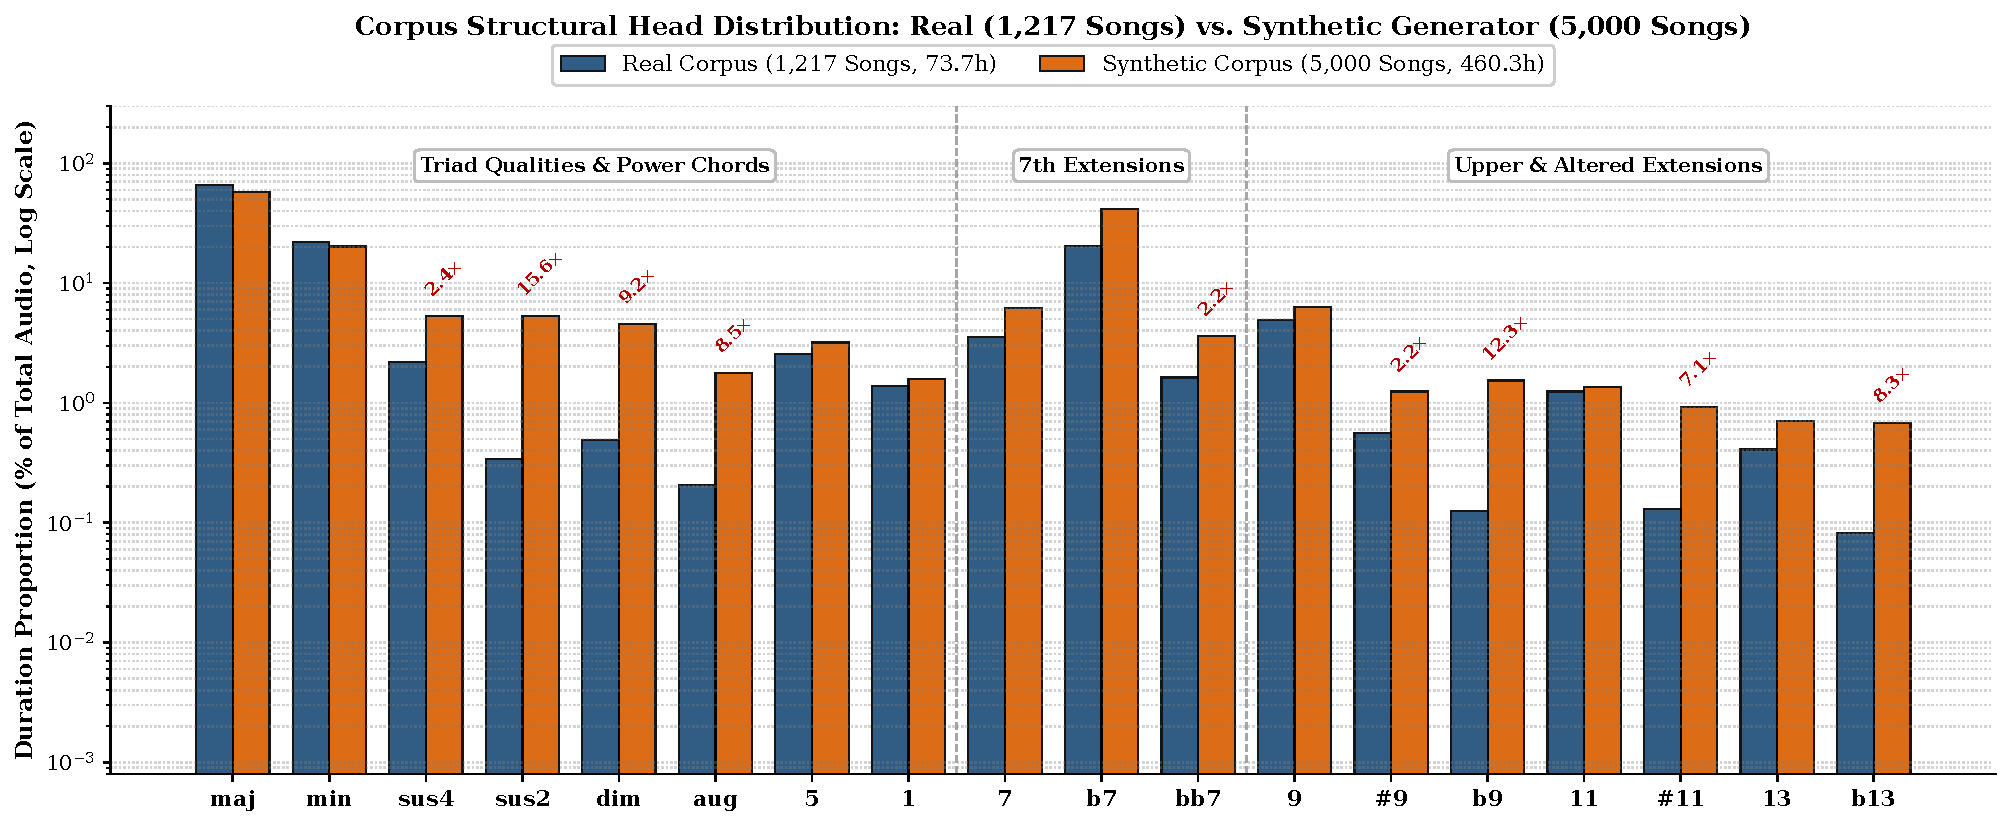
\includegraphics[width=0.74\textwidth]{figures/fig1_chord_distribution.pdf}
  \vspace{-7pt}
  \caption{Log-scale duration shares across 18 chord and extension classes in the $1{,}217$-song real benchmark ($73.7\,\text{h}$) versus our $5{,}000$-song synthetic corpus ($460.3\,\text{h}$, excluding \texttt{N}). Head~0 major ($65.75\%$) and minor ($22.16\%$) qualities occupy $87.91\%$ of non-silent real audio, leaving a steep Zipfian tail; quota scheduling expands rare triads ({\small\texttt{sus2}}: $0.34\% \!\to\! 5.31\%$, $15.6\times$; {\small\texttt{dim}}: $9.2\times$; {\small\texttt{aug}}: $8.5\times$; {\small\texttt{sus4}}: $2.4\times$) and upper extensions ({\small\texttt{b9}}: $12.3\times$; {\small\texttt{b13}}: $8.3\times$; {\small\texttt{\#11}}: $7.1\times$; {\small\texttt{\#9}}: $2.2\times$).}
  \label{fig:chord_dist}
  \vspace{-5pt}
\vspace{-1mm}
\end{figure*}

\subsection{Distribution-Shifted Harmonic Sampling}\label{subsec:harmonic_sampling}

Whereas AAM~\cite{ostermann2023aam} renders $3{,}000$ tracks from random diatonic triads ($\text{I}$--$\text{vi}$), omitting $\text{vii}^\circ$, suspended/augmented triads, and $7\text{th}$--$13\text{th}$ extensions~\cite{majchrzak2026training}, we design {\small\texttt{target\_corpus\_gen.py}} as a distributional intervention over $5{,}000$ tracks ($3{,}250$ pop/rock, $r_{\text{pop}} = 0.65$; $1{,}750$ jazz, $0.35$; $500{,}000$ events, $100$/track) along transitions extracted via ChoCo~\cite{deberardinis2023choco} from McGill Billboard~\cite{burgoyne2011expert} and Isophonics~\cite{mauch2009omras} ($1{,}114$ songs, $139{,}078$ events) plus the Weimar Jazz Database~\cite{pfleiderer2017inside} and iReal Pro\footnote{\url{https://www.irealpro.com}} ($2{,}477$ charts, $161{,}022$ events).

We parameterize each event $C_t$ by extending the 6-head space of Jiang et al.~\cite{jiang2019large} and ChordFormer~\cite{akram2026chordformer}: whereas both works restrict Head~0 to $6$ triad qualities ($73$ classes, $100$ logits)---omitting incomplete triads {\small\texttt{5}} and {\small\texttt{1}} in training and collapsing them into {\small\texttt{maj}} at evaluation---synthesizing standalone {\small\texttt{5}} and {\small\texttt{1}} exemplars allows us to expand Head~0 to $8$ qualities $q_t \in \{\text{\small\texttt{maj}}, \text{\small\texttt{min}}, \text{\small\texttt{sus4}}, \text{\small\texttt{sus2}}, \text{\small\texttt{dim}}, \text{\small\texttt{aug}}, \text{\small\texttt{5}}, \text{\small\texttt{1}}\}$ across roots $r_t \in \mathbb{Z}_{12}$ to form $S_t = (r_t, q_t)$ ($\hat{\mathbf{z}}_{0,t} \in \mathbb{R}^{97}$ with {\small\texttt{N}}); bass $b_t = (r_t + \Delta_{\text{bass},t}) \bmod 12$ for $\Delta_{\text{bass},t} \in \mathbb{Z}_{12}$ ($\hat{\mathbf{z}}_{1,t} \in \mathbb{R}^{13}$); and $\mathbf{E}_t = (e_{7,t}, e_{9,t}, e_{11,t}, e_{13,t})$ spans $\{\text{\small\texttt{N}}, \text{\small\texttt{7}}, \text{\small\texttt{b7}}, \text{\small\texttt{bb7}}\}$ ($\hat{\mathbf{z}}_{2,t} \in \mathbb{R}^4$, mapping {\small\texttt{dim7}} and, following ChordFormer~\cite{akram2026chordformer}, {\small\texttt{maj6}}/{\small\texttt{min6}} to {\small\texttt{bb7}}; Jiang et al.~\cite{jiang2019large} instead map the sixth to the 13th head), $\{\text{\small\texttt{N}}, \text{\small\texttt{9}}, \text{\small\texttt{\#9}}, \text{\small\texttt{b9}}\}$ ($\hat{\mathbf{z}}_{3,t} \in \mathbb{R}^4$), $\{\text{\small\texttt{N}}, \text{\small\texttt{11}}, \text{\small\texttt{\#11}}\}$ ($\hat{\mathbf{z}}_{4,t} \in \mathbb{R}^3$), and $\{\text{\small\texttt{N}}, \text{\small\texttt{13}}, \text{\small\texttt{b13}}\}$ ($\hat{\mathbf{z}}_{5,t} \in \mathbb{R}^3$), totaling $124$ logits. Per song ($4/4$ meter), we sample tonic $k \sim U_{\mathbb{Z}}(0, 11)$ ($S_1 \in \{\text{\small\texttt{0\_major}}, \text{\small\texttt{0\_minor}}\}$), $\text{BPM} \sim U_{\mathbb{Z}}(60, 180)$, and durations $d_t \in \{8, 6, 4, 3, 2, 1.5, 1\}$ ({\small\texttt{ww}}--{\small\texttt{q}}) with pop/rock weights $(.02, .03, .60, .05, .20, .05, .05)$ and jazz weights $(.01, .01, .30, .08, .40, .05, .15)$ ($\Delta t_{\text{sec}} = 60 d_t / \text{BPM}$).

In {\small\texttt{chord\_gen.py}}, sequence transitions factorize as:
\begin{equation}\label{eq:chord_factorization}
  \begin{split}
    P(C_t \!\mid\! C_{t-1}, C_{t-2}) &= P(S_t \!\mid\! S_{t-1}, S_{t-2})\,P(b_t \!\mid\! r_t, b_{t-1}) \\
    &\quad \cdot P(\mathbf{E}_t \!\mid\! S_t, b_t, \mathbf{E}_{t-1}).
  \end{split}
\end{equation}
Stage~1 interpolates order-2, order-1, and unigram tables via Witten-Bell weights $\lambda_i = n_i / (n_i + D)$ ($D = 25.0$):
\begin{equation}\label{eq:wb_backoff}
  \begin{split}
    P_{\text{final}}(S_t) &= \lambda_2 P_{\text{L2}}(S_t \!\mid\! S_{t-1}, S_{t-2}) + (1 - \lambda_2) \\
    &\quad \cdot \bigl[\lambda_1 P_{\text{L1}}(S_t \!\mid\! S_{t-1}) + (1 - \lambda_1) P_{\text{L0}}(S_t)\bigr],
  \end{split}
\end{equation}
using tempered $P_{\text{L1}} \propto P_{\text{raw}}^{1/\tau_1}$ ($\tau_{1,\text{pop}} = 2.2$, $\tau_{1,\text{jazz}} = 2.0$), floor $(1 - \epsilon) P_{\text{final}} + \epsilon P_{\text{L0}}$ ($\epsilon = 0.02$), and repeat discount $\delta = 0.20$ on $S_t = S_{t-1}$. Stage~2 applies order-1 bass backoff ($D = 25.0$), adds whole/half-note slash inversions at $p_{\text{inv}} = 0.10$ ($0.60$ $3\text{rd}$, $0.40$ $5\text{th}$), and slices sub-measure passing bass motion. Stage~3 walks a 4-slot prefix trie across state Trie~A ($N \ge 200$), triad Trie~B ($N \ge 500$), and genre Trie~C with $(b_t, \mathbf{E}_{t-1})$ backoff, merges enharmonic collisions ({\small\texttt{bb7+13}}, {\small\texttt{sus4+11}}, {\small\texttt{sus2+9}}, {\small\texttt{dim+\#11}}, {\small\texttt{aug+b13}}), and injects $p_{\text{NC}} = 0.01$ silence ({\small\texttt{N}}) solely on unextended root-position {\small\texttt{maj}}/{\small\texttt{min}} triads.

We partition tracks ($r_{\text{nat}} = 0.50$) into $2{,}500$ natural and $2{,}500$ targeted songs. For class $k$ with count $c_k$, quota $Q_k$ ($S_{\text{triad}} = 3.0\times$ on rare triads), event budget $N_{\text{ev}}$, and buffer $B \in \{50, 5{,}000\}$, due positions satisfy:
\begin{equation}\label{eq:quota_due}
  \text{pos}_{\text{due}}(k) = \left\lfloor \frac{(c_k + 1) N_{\text{ev}} + (Q_k + B) - 1}{Q_k + B} \right\rfloor,
\end{equation}
spaced by $\Delta_{\text{pos}} \ge 2$ along attested 1- or 2-step edges weighted by $P_{\text{dist1}}(s) C_{\text{local}}(s) / (1 + \text{RootCount}(s))$ ($3.38\times$--$95.8\times$ empirical upweighting). Versus the $1{,}217$-song corpus (Figure~\ref{fig:chord_dist}), duration shares rise across {\small\texttt{sus2}} ($0.34\% \!\to\! 5.31\%$, $15.55\times$), {\small\texttt{dim}} ($0.49\% \!\to\! 4.53\%$, $9.20\times$), {\small\texttt{aug}} ($0.21\% \!\to\! 1.77\%$, $8.50\times$), {\small\texttt{sus4}} ($2.21\% \!\to\! 5.28\%$, $2.40\times$), {\small\texttt{b7}} ($20.30\% \!\to\! 41.55\%$), {\small\texttt{bb7}} ($1.62\% \!\to\! 3.61\%$), {\small\texttt{b9}} ($0.13\% \!\to\! 1.54\%$, $12.28\times$), {\small\texttt{b13}} ($0.08\% \!\to\! 0.68\%$, $8.34\times$), {\small\texttt{\#11}} ($0.13\% \!\to\! 0.92\%$, $7.12\times$), {\small\texttt{\#9}} ($0.56\% \!\to\! 1.25\%$, $2.22\times$), {\small\texttt{9}} ($4.90\% \!\to\! 6.27\%$), {\small\texttt{13}} ($0.41\% \!\to\! 0.71\%$), and {\small\texttt{11}} ($1.25\% \!\to\! 1.36\%$).

\subsection{Symbolic Realization and Voicing Heuristics}\label{subsec:voicing}

Adapting AAM's four-stem JFugue paradigm~\cite{ostermann2023aam} ({\small\texttt{render.py}}), we map $4/4$ 16th-note grids ($4$ slots/beat) across: {\small\texttt{V0}} ($70\%$ pads, $30\%$ arpeggios), {\small\texttt{V1}} (bass in $[28, 55]$, $\text{E}_1$--$\text{G}_3$, playing roots, inversions, walking/passing lines, and $p_{\text{jump}} = 0.20$ octave leaps), {\small\texttt{V2}} (beam-search or random-walk melody masking $\{3, 4\}$ on {\small\texttt{sus2}}/{\small\texttt{sus4}}/{\small\texttt{1}} and restricting {\small\texttt{5}} to $\{0, 5, 7, 10\}$), and {\small\texttt{V9}} (Channel~10 drums).

Six policies parameterize {\small\texttt{V0}} MIDI bounds $[w_{\text{lo}}, w_{\text{hi}}]$ and voice limits $[V_{\text{min}}, V_{\text{max}}]$~\cite{tymoczko2011geometry}: {\small\texttt{pop-piano}} ($[43, 88]$, $[3, 7]$), {\small\texttt{pop-guitar}} ($[40, 76]$, $[3, 6]$), {\small\texttt{pop-synth}} ($[36, 96]$, $[3, 8]$), {\small\texttt{jazz-piano}} ($[48, 84]$, $[3, 6]$), {\small\texttt{jazz-guitar}} ($[45, 79]$, $[3, 5]$), and {\small\texttt{jazz-synth}} ($[40, 91]$, $[3, 7]$), with guitar policies enforcing $\le 4$-fret spans (cap $\le 12/15$) and barr\'e/drop shapes to prevent seventh-chord collapse across fretboard acoustics~\cite{nadar2019towards}. Unlike shell voicers that drop extensions, {\small\texttt{voicing/select.py}} enforces acoustic faithfulness: (1) $100\%$ of $7\text{th}$--$13\text{th}$ extensions sound in piano/synth policies, while guitar policies allow fallback only below Step~8 of an 8-level ladder at $+60.0 N_{\text{dropped}}$ penalty ($< 0.5\%$ drop rate); (2) the Distinguishing Chord Tone ($13\text{th} > 11\text{th} > 9\text{th} > 7\text{th} > 3\text{rd} > 5\text{th}$) avoids upper-root masking via top, isolated, or octave exposure; (3) $3\text{rds}$ never drop and $5\text{ths}$ omit ($p_{\text{omit\_5th}} \in [0.10, 0.70]$) only on {\small\texttt{maj}}/{\small\texttt{min}}; and (4) {\small\texttt{V0}} root omission ($p_{\text{omit\_root}} \in [0.02, 0.75]$) requires active {\small\texttt{V1}} bass. After low-interval and cluster pruning, we sample voicings via $P(c) \propto \exp(-(C(c) - \min C)/\tau_{\text{voic}})$ ($\tau_{\text{voic}} \in [2.2, 6.0]$) under:
\begin{equation}\label{eq:voicing_cost}
  \begin{split}
    C(c) &= w_{\text{vl}} d_{\text{vl}}(p_{\text{prev}}, p_c) - B_{\text{plr}} \\
    &\quad - 0.5 \min(|p_{\text{prev}} \cap p_c|, 3) + C_{\text{reg}}(c),
  \end{split}
\end{equation}
combining minimal voice-leading distance $d_{\text{vl}}$~\cite{tymoczko2006geometry,eitel2024perception} (solved via Hungarian assignment; $w_{\text{vl}} \in [0.5, 1.6]$, unmatched penalty $[1.2, 2.5]$), Neo-Riemannian $\text{P}/\text{L}/\text{R}$ bonus $B_{\text{plr}} \in [0.4, 3.0]$~\cite{cohn1998introduction,douthett1998parsimonious}, and spacing/drift cost $C_{\text{reg}}$. Five arpeggio profiles (gate $0.65$--$1.75$, velocity $78$--$96$) and {\small\texttt{HumanizedMidiRenderer.java}} prevent block-onset overfitting via $\sigma_t = 15.0\,\text{ms}$ jitter, pocket offsets ($0, +8, -4, -6, +2\,\text{ms}$ on pads, {\small\texttt{V1}}, {\small\texttt{V2}}, arpeggios, {\small\texttt{V9}}), $7.0\,\text{ms}$/string strums (GM~$24$--$31$), CC64 sustain (GM~$0$--$7$), and Gaussian velocity noise ($\sigma_v = 8.0$ harmonic; $\sigma_v = 4.0$ atop drum hits $\mathcal{N}(100, 8^2)$ kick/snare/crash, $\mathcal{N}(65, 8^2)$ ghost snare, $\mathcal{N}(80, 12^2)$ hi-hat/ride).

\subsection{Synthesis and Random-Mix Augmentation}\label{subsec:random_mix}

We synthesize stems via FluidSynth at $f_s = 22{,}050\,\text{Hz}$ ($16$-bit FLAC), rotating across four GM {\small\texttt{.sf2}} banks: {\small\texttt{FluidR3\_GM}} ($141\,\text{MB}$), {\small\texttt{MuseScore\_\allowbreak General\_\allowbreak Full}} ($468\,\text{MB}$), {\small\texttt{GeneralUser\_\allowbreak GS}} ($31\,\text{MB}$), and {\small\texttt{TimGM6mb}} ($5.7\,\text{MB}$). GM pools span $40$ {\small\texttt{V0}} patches ($16$ keyboard/organ/mallet, $12$ guitar/plucked, $12$ synth/pad), $13$ weighted {\small\texttt{V1}} bass patches (GM~$33, 34, 32, 35$ weighted $35, 25, 20, 15$), $18$ {\small\texttt{V2}} lead patches ($\ge 25\%$ vocal formants GM~$52$--$54$ in pop/rock), and randomized drum kits ($p = 0.60$ crash).

To mitigate acoustic overfitting, we mix stems via {\small\texttt{project\_\allowbreak condition\_\allowbreak corpus.py}} using Bernoulli dropout on {\small\texttt{V2}} and {\small\texttt{V9}} ($P = 0.70$ each: $49\%$ four-stem, $21\%$ {\small\texttt{cbm}}, $21\%$ {\small\texttt{cbp}}, $9\%$ {\small\texttt{cb}}) and perturb nominal gains $(0.0, +1.0, -1.0, -1.5)\,\text{dB}$ by $\Delta G_{\text{V0}}, \Delta G_{\text{V1}} \sim U(-3, +3)\,\text{dB}$, $\Delta G_{\text{V2}} \sim U(-3, +4)\,\text{dB}$, and $\Delta G_{\text{V9}} \sim U(-4, +4)\,\text{dB}$. FFmpeg applies {\small\texttt{V1}} saturation ($x - 0.05x^3$), $120\,\text{Hz}$ shelf ($+2.0\,\text{dB}$), and $3.5\,\text{kHz}$ low-pass; {\small\texttt{V0}} power-chord overdrive and cabinet EQ ($-3.0, +2.5, -6.0\,\text{dB}$ at $0.1, 0.25, 4.5\,\text{kHz}$); stereo panning ($60/40$ {\small\texttt{V0}}, $50/50$ {\small\texttt{V2}}, $40/60$ {\small\texttt{V9}}); split-band room convolution ($1.2/0.8/0.4\,\text{s}$, $82\%/18\%$ dry/wet, $150\,\text{Hz}$ wet high-pass); detuning $\Delta f_{\text{cents}} \sim U(-25, +25)\,\text{cents}$; $\pm U(1.5, 3.0)\,\text{dB}$ tilt at $1.5\,\text{kHz}$; console saturation ($x - 0.1x^3$); bus compression ($20/150\,\text{ms}$); and $-18.0\,\text{LUFS}$ normalization ($-1.0\,\text{dBTP}$ ceiling). This forces the Conformer~\cite{gulati2020conformer,akram2026chordformer} to extract timbre-invariant pitch-class profiles across polyphonic masking and detuned CQT bins. Across all $5{,}000$ tracks ($460.3\,\text{h}$), {\small\texttt{start\_\allowbreak padding\_\allowbreak frames=0}} anchors sample~$0$ to $t = 0.000\,\text{s}$, exporting frame-exact Harte {\small\texttt{.lab}} labels~\cite{harte2005symbolic} free of human annotation subjectivity~\cite{koops2019annotator}.
\section{Experimental Setup}\label{sec:experiments}

\subsection{Audio Preprocessing and ChordFormer-Variant Architecture}\label{subsec:preprocessing_arch}

Audio is downmixed to mono at $f_s = 22{,}050\,\text{Hz}$~\cite{akram2026chordformer}. We extract hybrid CQT spectrograms~\cite{brown1991calculation} with hop $H = 512\,\text{samples}$ ($\Delta t = 23.22\,\text{ms}$), window $N_{\text{win}} = 8{,}192\,\text{samples}$, and $b = 36\,\text{bins/octave}$ ($33.3\,\text{cents/bin}$) spanning $F_{\text{raw}} = 288\,\text{bins}$ ($8.0\,\text{octaves}$) from $f_{\min} = 23.12\,\text{Hz}$ ($\text{F}\sharp_0$, $A_4 = 440.0\,\text{Hz}$). Online pitch shifting steps across $[-5, +6]$ semitones on a $3$-bin grid, slicing $F = 252\,\text{bins}$ ($7.0\,\text{octaves}$, $\text{C}_1 = 32.70\,\text{Hz}$ to $\text{B}_7 = 3{,}951.07\,\text{Hz}$). Log-amplitude scaling clips to $[-80.0, 0.0]\,\text{dB}$, and right-zero-padding by $4\,\text{bins}$ yields $d_{\text{in}} = 256\,\text{channels}$ ($\mathbf{x} \in \mathbb{R}^{B \times T \times 256}$).

Our {\small\texttt{confor\_head16.py}} modifies ChordFormer~\cite{akram2026chordformer} ($N_L = 4$ Conformer blocks~\cite{gulati2020conformer}, $d_{\text{model}} = 256$, $p_{\text{drop}} = 0.10$): (1) half-step $\text{FFN}_1$ ($d_{\text{ffn}} = 1{,}024$); (2) depthwise convolution ($K = 31\,\text{frames} \approx 720\,\text{ms}$, pad $15$, Pointwise $256 \!\to\! 512 \!\to\! \text{GLU}$, Depthwise $256$, 1-group GroupNorm, SiLU, Pointwise $256 \!\to\! 256$, {\small\texttt{convolution\_first=True}}); (3) 16-head $\text{MHSA}$ ($h = 16$, $d_k = 16$); (4) half-step $\text{FFN}_2$; and (5) LayerNorm. Unlike the original~\cite{akram2026chordformer} ($h = 4$, BatchNorm, MHSA-first, relative positional encoding, {\small\texttt{triad\_limit=6}}, $100$ logits), we use $h = 16$, GroupNorm, convolution-first ordering, no positional encoding, and {\small\texttt{triad\_limit=8}} ($\hat{\mathbf{z}}_t = [\hat{\mathbf{z}}_{0,t}^{(97)} \mid \hat{\mathbf{z}}_{1,t}^{(13)} \mid \hat{\mathbf{z}}_{2,t}^{(4)} \mid \hat{\mathbf{z}}_{3,t}^{(4)} \mid \hat{\mathbf{z}}_{4,t}^{(3)} \mid \hat{\mathbf{z}}_{5,t}^{(3)}] \in \mathbb{R}^{124}$, Section~\ref{subsec:harmonic_sampling}; $|\Theta| = 6{,}123{,}644$); thus our metrics are not directly comparable to those reported in~\cite{akram2026chordformer}.

During inference ({\small\texttt{extractors/xhmm\_ismir.py}}), posteriors $\mathbf{p}_{h,t} = \text{Softmax}(\hat{\mathbf{z}}_{h,t})$ are decoded via linear-chain CRF Viterbi smoothing over Harte templates~\cite{harte2005symbolic,akram2026chordformer}:
\begin{equation}\label{eq:viterbi_decoding}
  \begin{split}
    S^*(t) = \arg\max_{c} \Bigl\{ &\max_{c'} \left( V(t-1, c') - \tau_{\text{crf}} \cdot \mathbb{I}(c' \neq c) \right) \\
    &+ \log P(c \!\mid\! \mathbf{x}_t) \Bigr\},
  \end{split}
\end{equation}
with $\tau_{\text{crf}} = 2.0$ (multi-head) and $\tau_{\text{crf}} = 30.0$ (MIREX). The CRF suppresses spurious frame-level fluctuations while preserving true harmonic boundaries.

\begin{table*}[t]
\centering
\footnotesize
\renewcommand{\arraystretch}{0.88}
\vspace{-8pt}
\caption{5-fold macro recall and $F_1$ (\%) across the 6 structural classification heads and isolated triad quality subsets (mean $\pm$ std across splits $s_0$--$s_4$). Control: 1,217-song real baseline; Experimental: 5,000-song synthetic pretraining + real finetuning ($\Delta = \text{Exp.} - \text{Control}$).}
\label{tab:head_metrics}
\vspace{1pt}
\begin{tabular}{lcccccc}
\toprule
\textbf{Structural Output Head} & \textbf{Control Rec. (\%)} & \textbf{Exp. Rec. (\%)} & \textbf{$\Delta$ Rec.} & \textbf{Control $F_1$ (\%)} & \textbf{Exp. $F_1$ (\%)} & \textbf{$\Delta$ $F_1$} \\
\midrule
\multicolumn{7}{l}{\textit{Primary 6-Head Multi-Task Decomposition:}} \\
  Root + Triad (97 classes)                     & 41.21 $\pm$ 3.12 & \textbf{42.66 $\pm$ 2.59} & +1.45 & 36.57 $\pm$ 2.07 & \textbf{36.70 $\pm$ 1.68} & +0.13 \\
  Bass Pitch (13 classes)                       & \textbf{84.81 $\pm$ 1.73} & 82.93 $\pm$ 1.51 & -1.88 & \textbf{84.72 $\pm$ 1.77} & 83.01 $\pm$ 1.57 & -1.70 \\
  7th Extension (4 classes)                     & \textbf{62.69 $\pm$ 4.27} & 62.55 $\pm$ 3.14 & -0.14 & \textbf{57.67 $\pm$ 2.73} & 56.99 $\pm$ 1.48 & -0.67 \\
  9th Extension (4 classes)                     & 35.33 $\pm$ 2.68 & \textbf{43.58 $\pm$ 7.54} & +8.25 & 34.98 $\pm$ 2.96 & \textbf{39.01 $\pm$ 6.25} & +4.03 \\
  11th Extension (3 classes)                    & 38.74 $\pm$ 7.85 & \textbf{41.71 $\pm$ 8.03} & +2.97 & 37.35 $\pm$ 3.60 & \textbf{42.14 $\pm$ 7.04} & +4.79 \\
  13th Extension (3 classes)                    & \textbf{35.36 $\pm$ 3.74} & 34.26 $\pm$ 1.95 & -1.10 & \textbf{36.09 $\pm$ 4.82} & 34.47 $\pm$ 2.47 & -1.62 \\
\midrule
  Macro Average (6 Heads)                       & 49.69 $\pm$ 2.10 & \textbf{51.28 $\pm$ 1.94} & +1.59 & 47.90 $\pm$ 1.69 & \textbf{48.72 $\pm$ 1.86} & +0.82 \\
\midrule
\multicolumn{7}{l}{\textit{Targeted Triad Quality Breakdown:}} \\
  Triad Quality (8 qualities + N)               & 50.23 $\pm$ 4.53 & \textbf{53.42 $\pm$ 3.96} & +3.19 & 45.52 $\pm$ 3.40 & \textbf{46.91 $\pm$ 2.57} & +1.39 \\
  Common Triads (\textit{maj}, \textit{min})    & \textbf{84.74 $\pm$ 1.97} & 83.08 $\pm$ 1.44 & -1.66 & \textbf{86.99 $\pm$ 1.19} & 86.05 $\pm$ 0.85 & -0.94 \\
  Rare Triads (\textit{sus2}, \textit{sus4}, \textit{dim}, \textit{aug}) & 41.67 $\pm$ 7.30 & \textbf{48.31 $\pm$ 6.47} & +6.64 & 53.11 $\pm$ 8.62 & \textbf{60.94 $\pm$ 6.26} & +7.83 \\
\bottomrule
\end{tabular}
\vspace{-2mm}
\end{table*}

\subsection{Datasets and Cross-Validation Protocol}\label{subsec:datasets_splits}

Our experimental workflow employs two corpora: (1) \textbf{Synthetic Pretraining Corpus}, used exclusively for pretraining and curriculum replay, comprising $5{,}000$ procedural random-mix tracks from Section~\ref{sec:generator} ($460.3\,\text{h}$, $21.8\,\text{GB}$ CQT HDF5; $4{,}500$ train and $500$ val tracks, seed \texttt{42}); and (2) \textbf{Real Benchmark Corpus}, the $1{,}217$-song collection spanning $731$ McGill Billboard, $287$ USPop2002/MARL, and $199$ Isophonics (Beatles/Queen) tracks. The final test set is drawn exclusively from this $1{,}217$ real-song collection (synthetic audio is never used for evaluation, and test-fold audio is never used for training); however, because our single pretraining corpus extracts symbolic transitions from full ChoCo Billboard/Isophonics tables and calibrates quotas against the $1{,}217$-song class prior (Figure~\ref{fig:chord_dist}), progression statistics from test-fold songs are not isolated from the generator. Under 5-fold cross-validation (seed \texttt{20190326}), splits \texttt{s0}--\texttt{s4} partition the $1{,}217$ real tracks ($730/731$ train, $243$ val, $243/244$ test tracks/fold; $11{,}436{,}357$ frames, $73.7\,\text{h}$), where Fold~0 {\small\texttt{maj}} ($4{,}465{,}981$ frames) and {\small\texttt{min}} ($1{,}586{,}913$) outnumber {\small\texttt{sus4}} ($30.5\!:\!1$), {\small\texttt{dim}} ($133.2\!:\!1$), {\small\texttt{sus2}} ($217.5\!:\!1$), {\small\texttt{aug}} ($292.4\!:\!1$), {\small\texttt{\#9}} ($221.8\!:\!1$), {\small\texttt{b9}} ($705.2\!:\!1$), {\small\texttt{\#11}} ($1{,}113.1\!:\!1$), and {\small\texttt{b13}} ($1{,}159.3\!:\!1$).

\subsection{Training Regimens: Baseline vs. Sim-to-Real Curriculum}\label{subsec:training_regimens}

We compare two regimens under FP16 mixed precision and AdamW ($\beta_1=0.9, \beta_2=0.999$) on $T = 1{,}000$-frame chunks ($23.22\,\text{s}$): (1) \textbf{Control Baseline} ({\small\texttt{control-\allowbreak benchmark}}), trained from scratch on the $1{,}217$ real songs for $24$ epochs/fold ($B=36$ or $48$, uniform LR $\eta$ over $\{10^{-3}\!:\!12, 10^{-4}\!:\!8, 10^{-5}\!:\!4\}$ epochs, $[-5, +6]$ pitch shifting); and (2) \textbf{Sim-to-Real Curriculum} ({\small\texttt{finetuned-\allowbreak benchmark}}), pretraining in Stage~1 ({\small\texttt{pretrain\_synthetic.py}}) on $5{,}000$ synthetic tracks for $7$ epochs ($10{,}500$ mini-batches, $B=36$, LR $\{10^{-3}\!:\!4, 10^{-4}\!:\!2, 10^{-5}\!:\!1\}$) with unweighted cross-entropy, pitch shifting, and SpecAugment~\cite{park2019specaugment} ($2$ frequency masks $\le 24\,\text{bins}$, $2$ time masks $\le 60\,\text{frames}$ at $-80.0\,\text{dB}$), then finetuning in Stage~2 ({\small\texttt{finetune\_real\_fold.py}}) on each real fold for $24$ epochs ($B=36$, LR $\{10^{-4}\!:\!12, 10^{-5}\!:\!8, 10^{-6}\!:\!4\}$).

Real training minimizes $\mathcal{L}_{\text{total}} = \sum_{h=0}^5 \lambda_h \mathcal{L}_h(\hat{\mathbf{z}}_h, \mathbf{y}_h; \mathbf{w}_h)$ ($\boldsymbol{\lambda} = [1, 1, 1, 1, 1, 1]$) with inverse-frequency class weights~\cite{jiang2019large,akram2026chordformer}:
\begin{equation}\label{eq:class_reweighting}
  w_{h, c} = \min \left( \left( \frac{\max_k N_{h, k}}{\max(N_{h, c}, 1.0)} \right)^{\alpha}, C_{\max} \right),
\end{equation}
using $\alpha = 0.50$, $C_{\max} = 10.0$, and clamps ($w_{2,\text{\small\texttt{b7}}} \approx 3.602$, $w_{3,\text{\small\texttt{9}}} = 6.000$, $w_{\text{\small\texttt{sus4}}} \ge 6.800$, $w_{\text{\small\texttt{5}}} \ge 6.000$, $w_{\text{\small\texttt{min}}} \ge 2.000$). Stage~2 adds: (1) \textbf{Inverted Discriminative LR} ($\mathbf{s}_{\text{lr}} = [0.2, 0.5, 1.0]$), scaling bottom blocks (Layers~0--1) by $0.2\eta$, top blocks (Layers~2--3) by $0.5\eta$, and output heads by $1.0\eta$; and (2) \textbf{Floor Curriculum Replay}, injecting SpecAugmented synthetic chunks at $\rho(\eta) = 0.150$ ($\eta \ge 10^{-4}$), $0.125$ ($\eta = 10^{-5}$), and a strict floor $\rho_{\min} = 0.100$ ($\eta \le 10^{-6}$) against catastrophic forgetting.
\section{Results and Discussion}\label{sec:results}

\subsection{Structured Head-Wise Recall and Rare-Class Gains}\label{subsec:head_wise_results}

Table~\ref{tab:head_metrics} summarizes 5-fold performance ($\tau_{\text{crf}} = 2.0$) of our ChordFormer variant across the six heads over all $11{,}436{,}357$ test frames (Section~\ref{subsec:preprocessing_arch}). Across the 6-head macro average, our Sim-to-Real curriculum raises recall from $49.69 \pm 2.10\%$ to $51.28 \pm 1.94\%$ ($+1.59\,\text{pp}$) and macro $F_1$ from $47.90 \pm 1.69\%$ to $48.72 \pm 1.86\%$ ($+0.82\,\text{pp}$), concentrating gains on sample-starved classes.

On Head~0 (Root + Triad, $97$ classes), macro recall increases from $41.21 \pm 3.12\%$ to $42.66 \pm 2.59\%$ ($+1.45\,\text{pp}$) and $F_1$ from $36.57 \pm 2.07\%$ to $36.70 \pm 1.68\%$ ($+0.13\,\text{pp}$), driven by non-diatonic structures: overall triad recall rises from $50.23 \pm 4.53\%$ to $53.42 \pm 3.96\%$ ($+3.19\,\text{pp}$; $F_1$ $45.52 \pm 3.40\% \!\to\! 46.91 \pm 2.57\%$). While common triads ({\small\texttt{maj}}, {\small\texttt{min}}) shift by $-1.66\,\text{pp}$ in recall ($84.74 \pm 1.97\% \!\to\! 83.08 \pm 1.44\%$) and $-0.94\,\text{pp}$ in $F_1$ ($86.99 \pm 1.19\% \!\to\! 86.05 \pm 0.85\%$), rare triads ({\small\texttt{sus2}}, {\small\texttt{sus4}}, {\small\texttt{dim}}, {\small\texttt{aug}}) increase from $41.67 \pm 7.30\%$ to $48.31 \pm 6.47\%$ in recall ($+6.64\,\text{pp}$, $+15.9\%$ relative) and from $53.11 \pm 8.62\%$ to $60.94 \pm 6.26\%$ in $F_1$ ($+7.83\,\text{pp}$, $+14.7\%$ relative). Similarly, Head~3 (9th) recall increases from $35.33 \pm 2.68\%$ to $43.58 \pm 7.54\%$ ($+8.25\,\text{pp}$, $+23.4\%$ relative; $F_1$ $+4.03\,\text{pp}$ to $39.01 \pm 6.25\%$), and Head~4 (11th) rises from $38.74 \pm 7.85\%$ to $41.71 \pm 8.03\%$ ($+2.97\,\text{pp}$; $F_1$ $+4.79\,\text{pp}$ to $42.14 \pm 7.04\%$).

\begin{figure*}[!t]
  \centering
  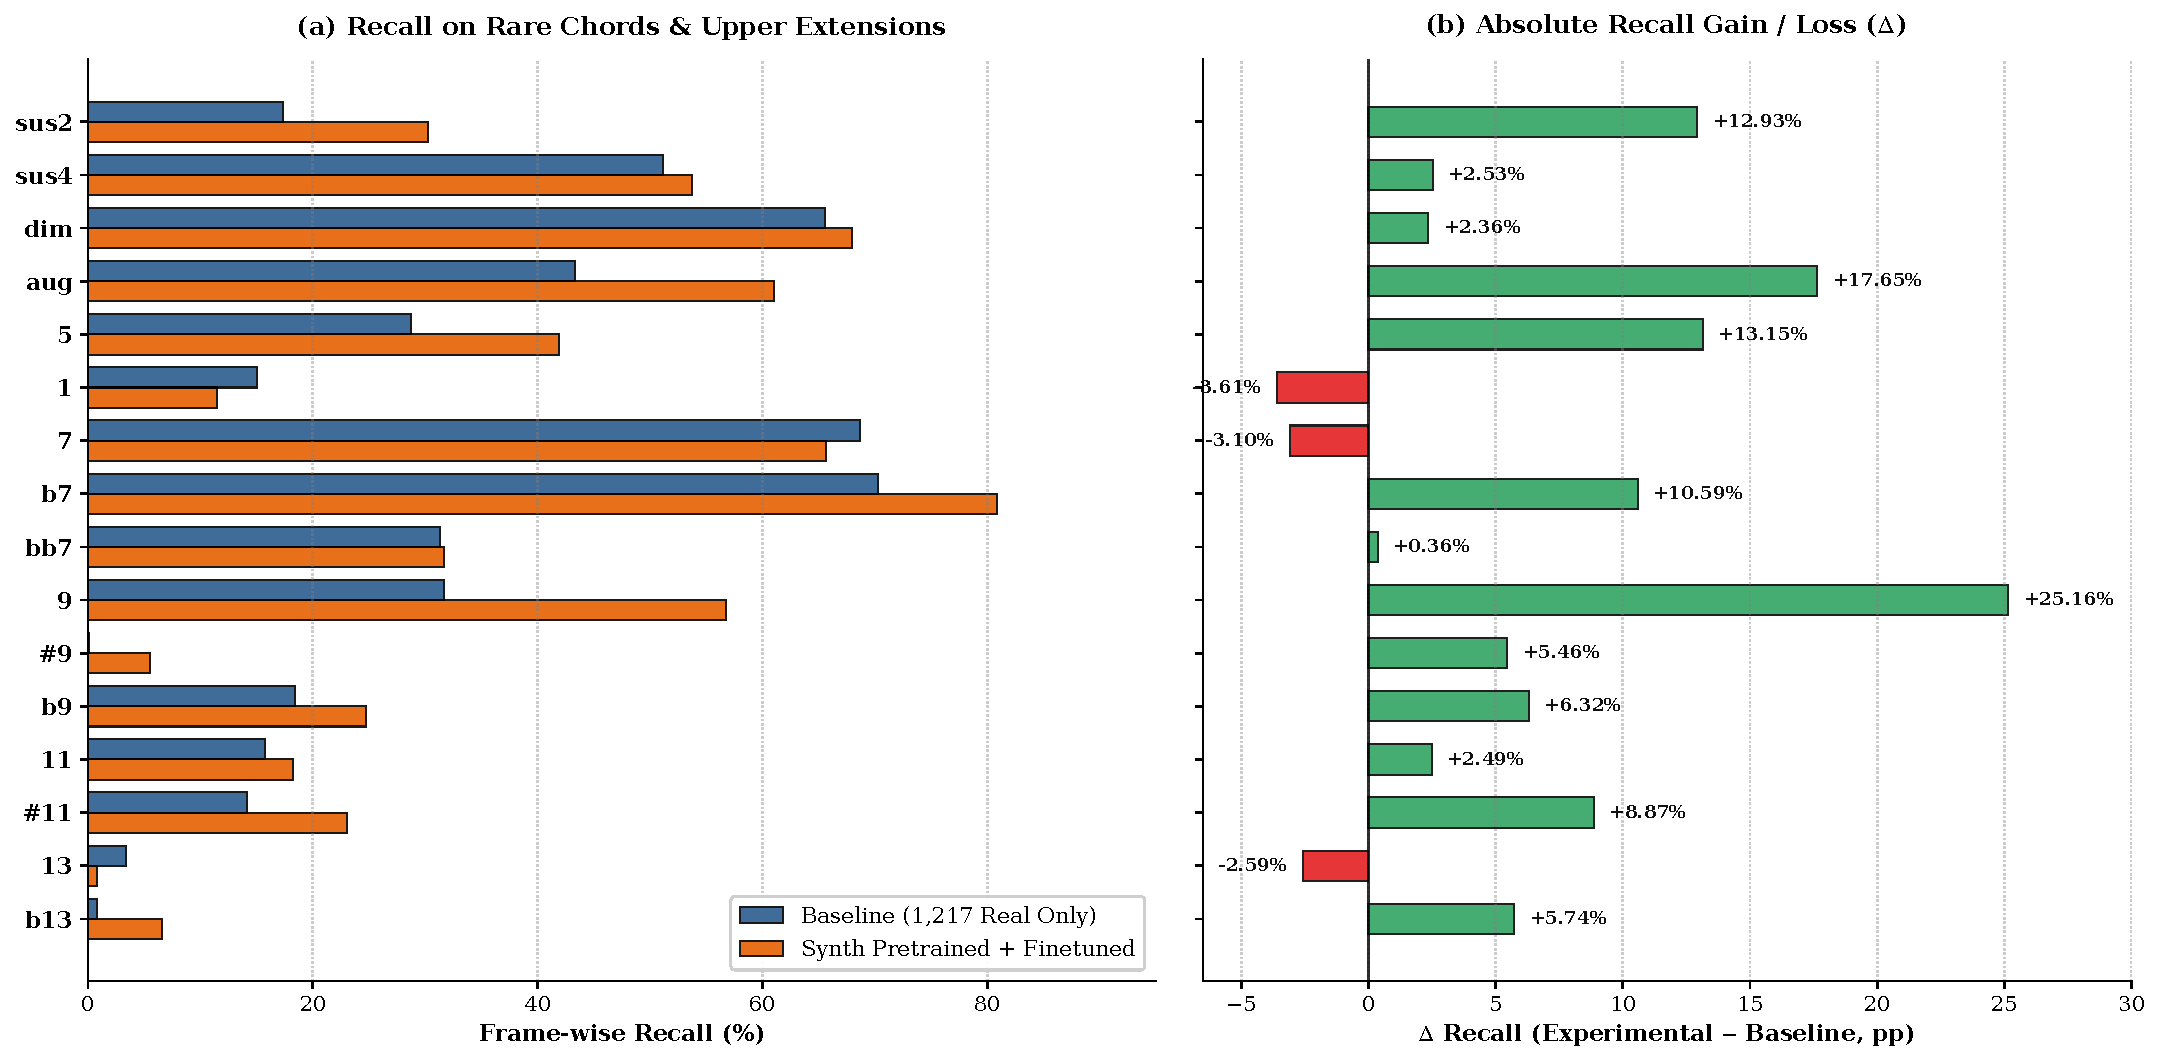
\includegraphics[width=0.68\textwidth]{figures/fig2_per_class_recall_delta.pdf}
  \vspace{-7pt}
  \caption{Per-class evaluation on rare triads, power chords, 7th extensions, and upper/altered extensions across $11{,}436{,}357$ frames of the $1{,}217$-song real benchmark: (a) absolute recall comparing Control Baseline (real-only) versus Experimental Curriculum (synthetic pretraining + real finetuning); (b) diverging recall gain ($\Delta\text{Recall}$), highlighting gains across {\small\texttt{9}} ($+25.16\,\text{pp}$), {\small\texttt{aug}} ($+17.65\,\text{pp}$), {\small\texttt{5}} ($+13.15\,\text{pp}$), {\small\texttt{sus2}} ($+12.93\,\text{pp}$), {\small\texttt{b7}} ($+10.59\,\text{pp}$), {\small\texttt{\#11}} ($+8.87\,\text{pp}$), {\small\texttt{b9}} ($+6.32\,\text{pp}$), {\small\texttt{b13}} ($+5.74\,\text{pp}$), and {\small\texttt{\#9}} ($+5.46\,\text{pp}$).}
  \label{fig:recall_delta}
  \vspace{-6pt}
\end{figure*}

Per-class metrics (Figure~\ref{fig:recall_delta}) show recall gains across most targeted rare qualities and extensions: {\small\texttt{aug}} recall rises from $43.37\%$ to $61.02\%$ ($+17.65\,\text{pp}$, $F_1$ $35.40\% \!\to\! 43.15\%$), {\small\texttt{sus2}} from $17.32\%$ to $30.25\%$ ($+12.93\,\text{pp}$, $F_1$ $17.40\% \!\to\! 19.90\%$), standalone {\small\texttt{5}} (uncollapsed from {\small\texttt{maj}}) from $28.76\%$ to $41.91\%$ ($+13.15\,\text{pp}$, $F_1$ $28.49\% \!\to\! 29.50\%$), {\small\texttt{dim}} from $65.61\%$ to $67.97\%$ ($+2.36\,\text{pp}$, $F_1$ $41.65\% \!\to\! 47.79\%$), {\small\texttt{sus4}} from $51.19\%$ to $53.72\%$ ($+2.53\,\text{pp}$), and {\small\texttt{b7}} from $70.31\%$ to $80.90\%$ ($+10.59\,\text{pp}$; {\small\texttt{bb7}} recall $+0.36\,\text{pp}$, $F_1$ $23.15\% \!\to\! 25.22\%$). On upper extensions, natural {\small\texttt{9}} rises $+25.16\,\text{pp}$ ($31.64\% \!\to\! 56.80\%$, $F_1$ $31.06\% \!\to\! 36.19\%$); {\small\texttt{\#9}} rises $+5.46\,\text{pp}$ ($0.07\% \!\to\! 5.53\%$, $F_1$ $0.10\% \!\to\! 4.97\%$); {\small\texttt{b9}} rises $+6.32\,\text{pp}$ ($18.39\% \!\to\! 24.71\%$, $F_1$ $9.56\% \!\to\! 18.02\%$); {\small\texttt{\#11}} rises $+8.87\,\text{pp}$ ($14.15\% \!\to\! 23.02\%$, $F_1$ $13.39\% \!\to\! 20.50\%$); and {\small\texttt{b13}} rises $+5.74\,\text{pp}$ ($0.84\% \!\to\! 6.58\%$, $F_1$ $0.77\% \!\to\! 8.43\%$). Conversely, recall regresses on bare-root {\small\texttt{1}} ($-3.61\,\text{pp}$), major {\small\texttt{7}} ($-3.10\,\text{pp}$), and natural {\small\texttt{13}} ($-2.59\,\text{pp}$, $3.35\% \!\to\! 0.76\%$).

While both regimens share identical inverse-frequency reweighting ($\alpha=0.50, C_{\max}=10.0$) in real training, contrasting the full Sim-to-Real curriculum against real-only training confounds synthetic pretraining with $7$ extra pretraining epochs, discriminative LRs, and replay; we hypothesize that physically voiced synthetic exemplars provide spectral diversity that loss reweighting on a few real tracks cannot.

\begin{table}[t]
\centering
\footnotesize
\renewcommand{\arraystretch}{0.88}
\setlength{\tabcolsep}{2.8pt}
\vspace{-8pt}
\caption{Weighted Chord Symbol Recall (WCSR, \%) across 5-fold cross-validation on 1,217 real songs ($s_0$--$s_4$, mean $\pm$ std). Control: 1,217-song real baseline; Experimental: synthetic pretraining + real finetuning.}
\label{tab:wcsr_mirex}
\vspace{1pt}
\begin{tabular*}{\columnwidth}{@{\extracolsep{\fill}}lccc@{}}
\toprule
\textbf{Evaluation Rule} & \textbf{Control (\%)} & \textbf{Experimental (\%)} & \textbf{$\Delta$ (pp)} \\
\midrule
  Root Pitch Only                  & \textbf{83.77 $\pm$ 1.88} & 82.30 $\pm$ 1.58 & -1.47 \\
  Major / Minor                    & \textbf{79.78 $\pm$ 2.38} & 77.04 $\pm$ 1.71 & -2.74 \\
  Major / Minor + Inversions       & \textbf{77.77 $\pm$ 2.22} & 75.17 $\pm$ 1.71 & -2.60 \\
  Triads (Full Quality)            & \textbf{75.01 $\pm$ 2.72} & 72.88 $\pm$ 1.97 & -2.13 \\
  Triads + Inversions              & \textbf{73.15 $\pm$ 2.58} & 71.13 $\pm$ 1.95 & -2.02 \\
  Sevenths (Standard)              & \textbf{66.46 $\pm$ 2.46} & 62.46 $\pm$ 1.73 & -4.00 \\
  Sevenths + Inversions            & \textbf{65.12 $\pm$ 2.42} & 61.18 $\pm$ 1.72 & -3.94 \\
  Tetrads (Extended)               & \textbf{61.62 $\pm$ 2.73} & 58.20 $\pm$ 1.74 & -3.42 \\
  Tetrads + Inversions             & \textbf{60.38 $\pm$ 2.69} & 57.02 $\pm$ 1.75 & -3.36 \\
\midrule
  \textbf{MIREX Metric (Overall)}  & \textbf{81.49 $\pm$ 2.56} & 79.59 $\pm$ 1.85 & -1.90 \\
\bottomrule
\end{tabular*}
\end{table}

\subsection{Standard Frame-Level WCSR and MIREX Evaluation}\label{subsec:wcsr_mirex}

Table~\ref{tab:wcsr_mirex} reports duration-weighted chord symbol recall (WCSR) via \texttt{mir\_eval.chord}~\cite{raffel2014mireval} ($\tau_{\text{crf}} = 30.0$). Across all ten comparison rules, the Sim-to-Real curriculum scores strictly lower than the real-only baseline: Root drops by $1.47\,\text{pp}$ ($83.77\% \!\to\! 82.30\%$), Major/Minor by $2.74\,\text{pp}$ ($79.78\% \!\to\! 77.04\%$; $-2.60\,\text{pp}$ with inversions), Triads by $2.13\,\text{pp}$ ($75.01\% \!\to\! 72.88\%$; $-2.02\,\text{pp}$ with inversions), Sevenths by $4.00\,\text{pp}$ ($66.46\% \!\to\! 62.46\%$), Tetrads by $3.42\,\text{pp}$ ($61.62\% \!\to\! 58.20\%$), and overall MIREX WCSR by $1.90\,\text{pp}$ ($81.49 \pm 2.56\% \!\to\! 79.59 \pm 1.85\%$).

We attribute this divergence to a precision-recall and metric-weighting trade-off: WCSR weights accuracy strictly by interval duration ($\sum_i d_i \mathbb{I}(\hat{C}_i == C_i) / \sum_i d_i$), biasing it toward unextended {\small\texttt{maj}} ($44.93\%$ of real duration) and {\small\texttt{min}} ($11.95\%$; $65.75\%$/$22.16\%$ on Head~0 with extensions). Under Harte recombination, candidate log-probabilities sum across all six heads ($\log P_k(t) = \log p_{\text{triad}} + \mathbb{I}(\text{use\_bass})\log p_{\text{bass}} + \sum_e \log p_e$). Expanding minority decision boundaries in $\hat{\mathbf{z}}_{h,t}$ to capture rare qualities and extensions inevitably introduces false-positive activations on acoustically ambiguous frames of dominant triads (e.g., guitar overtones or vocal passing tones triggering {\small\texttt{sus4}} or {\small\texttt{b7}}, where per-class $F_1$ shifts by $-1.79\,\text{pp}$ and $-0.89\,\text{pp}$ despite $+2.53\,\text{pp}$ and $+10.59\,\text{pp}$ recall gains). Because rare classes occupy minuscule duration slices ({\small\texttt{sus2}} $0.34\%$, {\small\texttt{aug}} $0.21\%$, {\small\texttt{b9}} $0.13\%$, {\small\texttt{b13}} $0.08\%$), true-positive detections on the harmonic tail yield negligible WCSR credit, whereas any false-positive excursion on a majority triad immediately penalizes duration overlap.

Stage~2 adaptation is intended to bound this trade-off. Updating linear heads at $1.0\eta$ while anchoring bottom Conformer blocks ($0.2\eta$) and maintaining the $\rho_{\min} = 0.10$ synthetic replay floor is designed to recalibrate output logit priors to studio mixes while retaining minority features. Moreover, synthetic pretraining lowers 5-fold WCSR standard deviation across all ten rules in Table~\ref{tab:wcsr_mirex} (MIREX $\pm 2.56\% \!\to\! \pm 1.85\%$; MajMin $\pm 2.38\% \!\to\! \pm 1.71\%$; Tetrads $\pm 2.73\% \!\to\! \pm 1.74\%$), consistent with narrower WCSR spread (though spread widens on sparse heads like 9ths in Table~\ref{tab:head_metrics}, $\pm 2.68\% \!\to\! \pm 7.54\%$).

\subsection{Sim-to-Real Acoustic Domain Gap and Extension Masking}\label{subsec:acoustic_domain_gap}

Bridging SoundFont synthesis to studio recordings requires overcoming static synthesis timbres and polyphonic overtone masking. Because encoders can memorize deterministic SoundFont attacks and envelopes, our random-mix pipeline applies Bernoulli stem dropout ($P=0.70$ on lead/drums), gain perturbations ($\Delta G \in [-4, +4]\,\text{dB}$), overdrive, split-band room convolution, and detuning ($\Delta f_{\text{cents}} \sim U(-25, +25)\,\text{cents}$), forcing Conformer blocks to learn timbre-invariant intervals across detuned CQT bins.

We also hypothesize that register and overtone alignment shape the per-class trends in Figure~\ref{fig:recall_delta}: (1) \textit{Low-Register Triads}: Rare triads ({\small\texttt{sus2}}, {\small\texttt{aug}}, {\small\texttt{dim}}) alter 3rd/5th degrees in $\text{C}_1$--$\text{C}_4$, where $36\,\text{bins/octave}$ CQTs resolve fundamentals ($+2.36\,\text{pp}$ to $+17.65\,\text{pp}$ recall), whereas bare-root {\small\texttt{1}} ($-3.61\,\text{pp}$) lacks tertian intervals to separate it from bass/melody octaves; (2) \textit{Natural Extensions} ({\small\texttt{7}}, {\small\texttt{11}}, {\small\texttt{13}}): In $\text{C}_4$--$\text{B}_6$, upper tones compete with vocal formants, guitars, and cymbals---natural {\small\texttt{11}} clashes with a major 3rd ($+2.49\,\text{pp}$), while major {\small\texttt{7}} ($-3.10\,\text{pp}$) and natural {\small\texttt{13}} ($-2.59\,\text{pp}$, $3.35\% \!\to\! 0.76\%$) have partials aligning with root/5th overtones; and (3) \textit{Altered Extensions} ({\small\texttt{\#9}}, {\small\texttt{b9}}, {\small\texttt{\#11}}, {\small\texttt{b13}}): Chromatic alterations diverge from the triad's overtone series, which may yield more isolated CQT peaks ($+5.46\,\text{pp}$ on {\small\texttt{\#9}}, $+5.74\,\text{pp}$ on {\small\texttt{b13}}).
\section{Conclusion}\label{sec:conclusion}

We presented a Sim-to-Real pretraining framework for large-vocabulary ACR synthesizing $5{,}000$ multitracks ($460.3\,\text{h}$) via empirical transition sampling, rare-chord quota scheduling, physically constrained voicings, and random-mix augmentation. Pretraining a ChordFormer variant on synthetic audio and finetuning via inverted discriminative learning rates ($\mathbf{s}_{\text{lr}} = [0.2, 0.5, 1.0]$) and floor curriculum replay ($\rho_{\min}=0.10$) improves recall over the real baseline on rare triads ($+6.64\,\text{pp}$), natural 9ths ($+25.16\,\text{pp}$), and alterations ($+5.46\,\text{pp}$ on {\small\texttt{\#9}}, $+5.74\,\text{pp}$ on {\small\texttt{b13}}) while narrowing 5-fold WCSR spread.\footnote{Code and models: \url{https://github.com/shojha24/probabilistic-composition-generator}; companion benchmark: \url{https://github.com/shojha24/ChordFormer-Artificial-Dataset-Benchmarking}.} Limitations include testing a single quota operating point, omitting an equal-compute control, and extracting generator transitions/priors from full ChoCo Billboard/Isophonics tables rather than per-fold training splits; future work will enforce fold-isolated extraction, add compute-matched ablations, tune quotas, and integrate DDSP.

\clearpage
\bibliography{references}

\end{document}
